
\chapter{Retrieval-Augmented Generation}
\label{sec:rag}

When the first LLMs were released, people were blast away by the numerous skills these models had learned. Yet, after a while it became clear that producing factually correct answers was a skill the models had not learned. It is not what the models were trained for and certainly when a fact was not in the training data, the LLM has no way of knowing that fact. Even worse, the LLM was trained to always give an answer, no matter how incorrect it is and it does so confidently. When an LLM makes up something rather than being based on facts, it is called a hallucination. These hallucinations can make the answers unreliable and Retrieval-Augmented Generation is made to solve that problem (partially).

\section{What is RAG?}

\begin{figure}[h]
	\centering
	\captionsetup{justification=centering}
	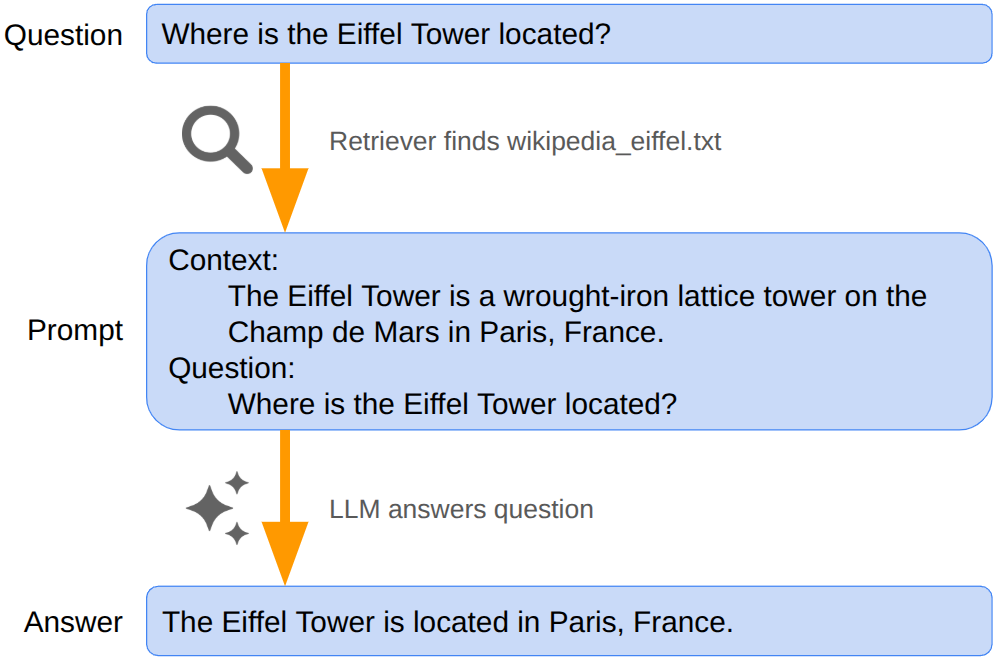
\includegraphics[width=0.6\linewidth]{fig/RAG.png}
	\caption{Diagram of the basic RAG pipeline.}
	\label{fig:rag}
\end{figure}

RAG is a system where the LLM is provided with factual information in a prompt, such that it can answer correctly even if it has never seen that fact before or already forgot about it. Practically, a simple RAG pipeline has two stages: retrieval and generation. First the user asks a question and the most relevant pieces of text are retrieved from a database of facts. Then, this information is given to the LLM as part of the prompt, before it answers the question. This is visualized in Figure \ref{fig:rag}.

\subsection{Retriever}
The retriever in a RAG pipeline refers to the component that takes query text as an input and returns the most relevant context chunks. Needless to say, a good retriever is the basis for a good RAG system. In practice, good retrievers are hybrid retrievers, that combine the advantages of a lexical search and a semantic search. Lexical search works on keywords and is good to find literal matches between the question and documents. This is complemented with dense retrieval, using an embedding model. An embedding model is a neural network that is trained to take text as input and transform it into a vector that contains the ``meaning'' of the text. For a first time reader, this might not sound intuitive. For the purposes of this thesis, it is only important to understand that this model creates an output for each piece of text, which we can easily compare. For example, given a query and a piece of context, we can say: these strings are 20\% similar. In other words, this embedding model will allow us to efficiently find which pieces of text in the entire database are semantically similar to the query. 

While lexical search is pracitally set in stone, there is much freedom in the semantic search. There are many strong embedding models available for general use cases, such as the Splade models \cite{formal2021splade, formal2021spladev2, lassance2024spladev3}, Contriever \cite{izacard2021unsupervisedcontriever}, GTR \cite{ni2021largegtr}, ... These could serve as a basis for fine-tuning on a specific domain, such as the medical domain for this thesis. However, within the scope of this thesis, we limit ourselves to using existing embedders directly. In that case, it is important to find the right embedder for the specific use case.

To objectively compare different models, it is important to choose the right metric for the job. In this thesis, the goal of the retriever is to get one piece of information and to make sure that piece is ranked as high as possible. The logical metrics to use in this case are Hit@k and Mean Reciprocal Rank (MRR). Hit@k is the probability that a relevant document is in the top k results. So Hit@3$=0.7$ means that a relevant document is in the top 3 retrieved documents for 70\% of the times. The MRR is defined as $\frac{1}{U} \sum_{u=1}^U \frac{1}{rank_i}$, with the rank defined as the place of first document that is relevant, as shown in Figure \ref{fig:rag_rank}. In the best case scenario, a relevant document is retrieved on place 1, resulting in rank 1. As the MRR is the mean of many such ranks, the best possible MRR is 1. Thus, the MRR ranges between 0 and 1.

\begin{figure}[h]
	\centering
	\captionsetup{justification=centering}
	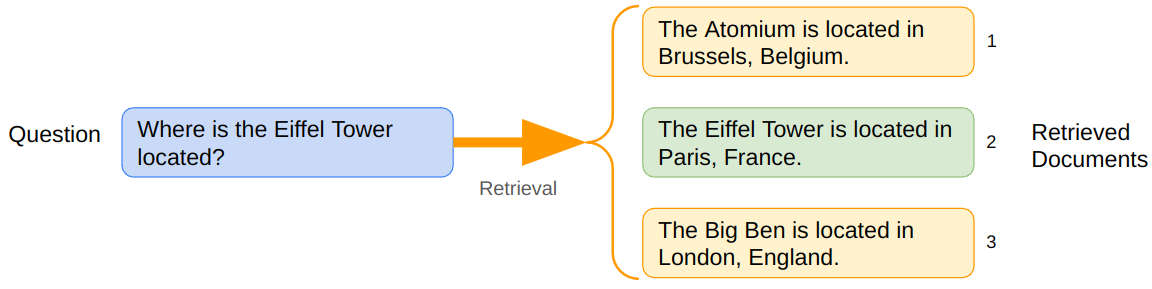
\includegraphics[width=0.9\linewidth]{fig/RAG_rank.png}
	\caption{Example of a retrieval to explain the rank. For this question, there is clearly one relevant document retrieved: the second one. This makes the rank of this retrieval 2.}
	\label{fig:rag_rank}
\end{figure}

\subsection{Generator}
The generator is the component that takes the question and context as input, to formulate an answer using the information in the context. In practice, the question and context are combined in a prompt and that prompt is fed to an LLM. The first step is optimized through prompt engineering. This has become a whole field of research in se and there are many ways to incentivise the LLM to give better answers. Common prompt engineering methods include: adding structure, adding examples, telling the LLM what not to answer, defining roles, ... The second step is just the LLM generating an answer, but that can also be optimized strongly by choosing the right LLM and/or fine-tuning. Again, for the scope of this thesis fine-tuning costs too much time and compute. Thus, we limit ourselves to choosing the optimal LLM for the use case.

\section{RAG optimizations}
A modern RAG pipeline may consists of many more stages than a simple retrieve and generate step. As each application requires different tricks, there is an endless amount of extra steps one could add. For this reason only the potentially interesting methods are summarized below.

\subsection{Pre-Retrieval}
\label{sec:pre_retrieval}
In an additional pre-retrieval step, the input of the user is first processed. As a normal user is not an experienced prompt engineer, the questions users ask are more often than not incomplete, ambiguous, ... To better interpret the question, three different methods have emerged: abstracting the question, retrieving based on hypothetical answer and splitting the question.

\subsubsection{Abstracting the question}

\begin{figure}[h]
	\centering
	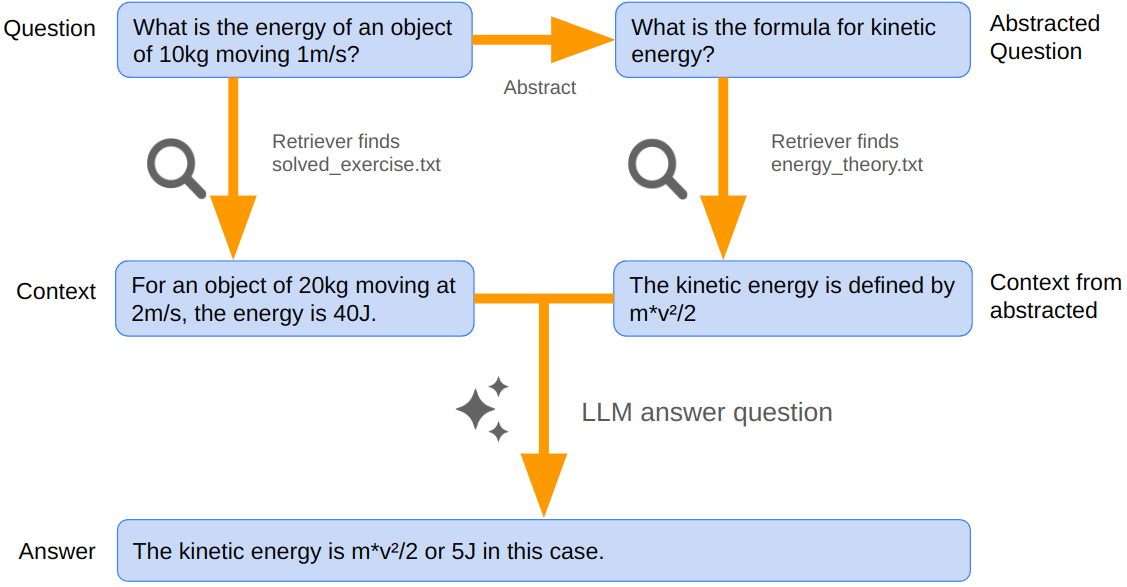
\includegraphics[width=0.9\linewidth]{fig/rag_abstract_prompt.png}
	\caption{Diagram of prompt abstraction. First, the prompt is abstracted to the higher level reasoning that is necessary to answer the question. Then the relevant context is searched for both the original question and the abstracted question. The contexts are combined to form the prompt for the LLM. So the left part of the diagram is basic RAG and the right part adds the abstracted question for retrieval. Note that this example is cherry-picked such that the "context from abstracted" is much better, but often times the direct retrieval also yields relevant context, depending on the question.}
	\label{fig:rag_abstract_prompt}
\end{figure}

Step-Back Prompting \cite{zheng2023takeastepback} tries to make the retrieval easier by first abstracting the question. The idea is that highly specific questions with uncommon words can confuse the retriever, preventing the it from finding semantically similar, relevant documents. This is also shown in Figure \ref{fig:rag_abstract_prompt}.

\subsubsection{Retrieving based on hypothetical answer}

\begin{figure}[h]
	\centering
	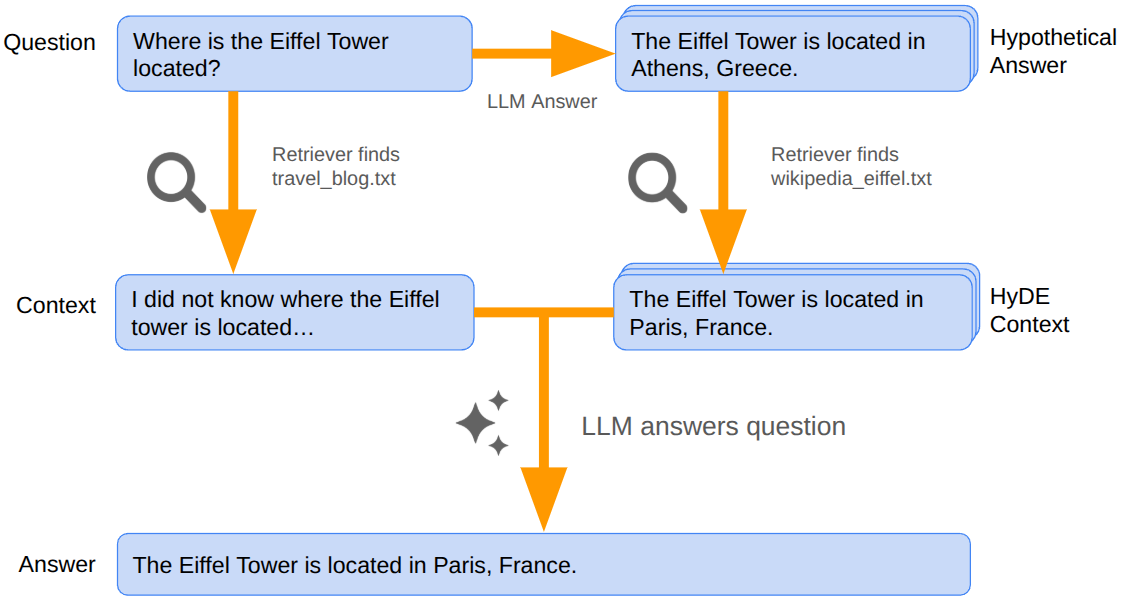
\includegraphics[width=0.9\linewidth]{fig/rag_hyde.png}
	\caption{Diagram of HyDE. First, the LLM is asked to answer the question. Then the relevant context is searched for both the original question and the hypothetical answer. The contexts are combined to form the prompt for the LLM. So the left part of the diagram is basic RAG and the right part adds the hypothetical answer for retrieval. Note that the example is again cherry-picked to clarify where HyDE excels.}
	\label{fig:rag_hyde}
\end{figure}

Retrieval is based on semantic similarity between the query and the context in the database. However, the question a user asks can be completely different from the expected answer. To narrow the gap between the query and the retrieved document, HyDE \cite{gao2023precisehyde} builds a hypothetical answer to the question. This hypothetical answer can contain hallucinations, but that is not a problem. The point is that the hypothetical answer should be semantically closer to the real answer than the question is. This is further clarified by Figure \ref{fig:rag_hyde}.

\subsubsection{Splitting the question}

\begin{figure}[h]
	\centering
	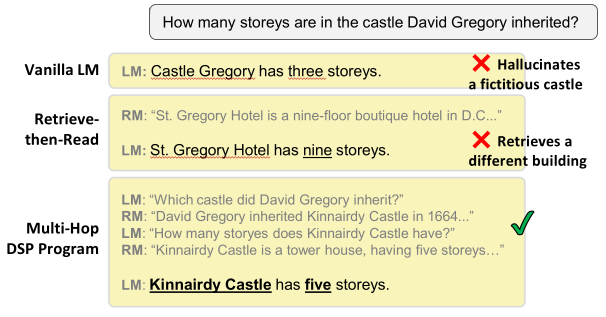
\includegraphics[width=0.7\linewidth]{fig/demonstrate_search_predict.png}
	\caption{Illustration from Demonstrate-Search-Predict \cite{khattab2022demonstrate}. Demonstrate-Search-Predict (DSP) performs multi-hop reasoning, retrieving the necessary documents in each step. This is indicated by the interleaving of LM (language model) asking questions and the RM (retrieval model) answering those questions by providing the right pieces of text.}
	\label{fig:demonstrate_search_predict}
\end{figure}

A question often consists of multiple subquestions. Demonstrate-Search-Predict \cite{khattab2022demonstrate} and IRCoT \cite{trivedi2022interleaving} try to leverage the chain of thought strategy, where the question is reduced to a simpler question iteratively. Figure \ref{fig:demonstrate_search_predict} clarifies this principle with an example. Later, each question will then be answered with its own relevant retrieved documents. More parallel methods like ToC \cite{kim2023tree} and RAG-Fusion \cite{rackauckas2024ragfusion} break down the question recursively into multiple questions. The difference with CoT is that there are now multiple branches.

\subsection{Post-retrieval}
The retrieval step typically yields multiple chunks, pieces of text, in which the answer is hopefully present. But sometimes the retriever fails and it adds an irrelevant chunk or it succeeds, but the relevant part is only a small fraction of the entire chunk. This all adds noise to the input of the LLM and LLMs often get confused by this. That is why a post-retrieval step is sometimes necessary to filter the abbundance of information. The two relevant methods to this thesis are prompt compression and reranking. Prompt compression is discussed later, as it also falls under the energy optimization methods.

\subsubsection{Reranker}
A reranker takes the retrieved contexts and orders them based on relevance. The difference with the embedder of a retriever, is that it does not go to an intermediary embedding space to define similarity. This usually makes it much more compute intensive, but also more accurate. For this reason, the reranker is only used after only a limited amount of candidate chunks remain.

QLM is a recent method that uses the modern LLM's zero-shot capabilities to rerank \cite{zhuang2023qlm}. The score of the context is the probability that the question would be generated given the context. The idea is that more relevant contexts should make the question more likely. Another method is to train a cross-encoder to output the relevance of the context given the query directly. One such cross-encoder is ``BGE-Reranker-v2-M3'' \cite{chen2024bge}.

\section{Generator energy optimization}
While the previous optimization techniques were about generating better answers, this section discusses how the best answer is generated with the least amount of energy. Speculative decoding is the method that is the main topic of this thesis, but we also list alternative methods that are equally valid to reduce the energy consumption of the generator. Unfortunately, energy consumption is rarely discussed in papers, so without actual experiments we only know that the method should be able to reduce energy usage in theory.

\subsection{Speculative decoding}
Speculative decoding tries to reduce the energy an LLM takes to generate an answer by reducing the number of forward passes ($\approx$ the number of times the LLM is activated). Less forward passes in the LLM mean not only less latency, but also less energy consumed. The key idea to speculative decoding is that when the output of an LLM is known, the LLM can verify all generated tokens in parallel, in one forward pass. However, to know the output, we need to use the LLM. This creates a chicken and egg problem, but it can be solved by guessing. First we guess the output of the LLM, not only for the next token, but also for further tokens. With that guess, all tokens are checked in parallel and only the correctly guessed tokens are kept. Needless to say, the open question is: how is a good guess made without calling the LLM itself and how much does that estimation itself cost. As speculative decoding is the main topic of this thesis the details go in to a separate Chapter \ref{sec:speculative_decoding}.

\subsection{Prompt compression}
Prompt compression intends to make the prompt, the input of the LLM, shorter, while still maintaining the meaning behind the prompt. There are multiple reasons to keep the length of the input for a LLM limited. Firstly, longer input increases the necessary computation, which leads to longer latency and more energy consumption \cite{kim2023arithmeticintensityllm}. Secondly, each model has a limited context window and it is impossible for the LLM process the full input when the input gets longer. Lastly, longer input can degrade the quality of the generation. This is because typically LLMs are trained with fixed length inputs, much shorter than the context window. Even though they are then trained somewhat to work with longer inputs, the performance usually stays subpar \cite{levy2024sameinputlength, liu2024lost}. To limit these effects, there are three categories of prompt compression, each with their own benefits and weaknesses: extractive compression, abstractive compression and token pruning.

\subsubsection{Extractive compression}
Extractive compression is the type highest performing compresion, and it is based on extracting relevant parts from the original text. These parts can have a granularity of phrases, sentences or passages? In RAG systems, this extraction can be based on the semantic similarity between a part of the context and the input prompt. 

Below, the most interesting methods for this thesis are described: CPC \cite{liskavets2025cpc}, RECOMP \cite{xu2023recomp} and Selective Context \cite{li2023selectivecontext}, ordered by relevance. CPC uses contrastive learning to fine-tune an embedder, such that it can find similarity between context sentences and the question asked. The authors noticed that embedders are good at finding direct answers to a question, but not components of answers, so they trained the embedder to learn similarity between questions and parts of answers. Only the relevant sentences are then kept and the irrelevant ones are cut out. RECOMP has a similar method of contrastive learning, but they get their positive samples from sentences that lower the perplexity of the ground truth answer the most. Selective Context uses a whole different strategy, where they combine the token-level perplexities to get a phrase level perplexity. The lowest perplexity phrases are then cut out.

\subsubsection{Abstractive compression}
In abstractive compression, the prompt is summarized by a smaller language model. This summary can contain new tokens that were not in the original prompt, unlike the other techniques. RECOMP \cite{xu2023recomp} approaches this task by training a small model to summarize like the modern LLMs do. It is important that the summarizing model is many times smaller than the LLM to actually make gains, rather than losses through overhead.

\subsubsection{Token pruning}
Token pruning exploits the fact that an LLM can handle input that is not exactly natural language. By cutting away tokens that were ``obvious'' to an LLM anyway, the compressor can condense information by cutting only the obvious tokens and leaving the surprising (read high perplexity) tokens as is. LLMLingua \cite{jiang2023llmlingua} laid the foundations of token compression for both LLMLingua 2 \cite{pan2024llmlingua2} and LongLLMLingua \cite{jiang2023longllmlingua}, which are currently the best token pruners. They are all based on the same principle of using a smaller model's perplexity to estimate the relevance of a token. Then, the low perplexity tokens are cut iteratively, recalculating perplexity every time. To get to the optimal compression level, a budget controller decides what perplexity is too low. While this method yields high compression ratios, a known issue is that an LLM often copies literal parts of the prompt. This means that the answer also contains text that is rather incoherent to humans, where some tokens were just dropped.

\subsection{Hybrid generation}
Certain pieces of text are easier to generate than others. In a RAG context, that could be when the LLM is quoting excerpts from the context. AutoMix tries to improve efficiency by generating these easier parts with a smaller LLM. This hybrid generation method works as follows. First, the smaller LLM generates verifiable statements from the RAG context. Then it is given a verification prompt and the probability of the ``Correct'' and ``Incorrect'' token are measured. If the probability that the statement is correct is too low, the task is passed to the large LLM do it better. Originally, this method was posed as a way to cut monetary costs, where the smaller LLM is local and the large LLM is paid for through API. Yet, this method has potential to reduce both latency and energy consumption.

\iffalse

Post-generation
Source highlighting
	Source highlighting via constrained decoding (ask LLM which source it used)
	https://huggingface.co/learn/cookbook/en/structured\_generation
	Finetuning SLM to quote sources
https://community.openai.com/t/source-document-chunk-identification-and-highlighting-for-rag-usecase/883302/2
Post-hoc semantic search?
Loop
FLARE
	Retrieve when generated sentence has low probability tokens
Self-RAG
	Generate retrieval tokens (needs finetuning)
Adaptive RAG
Train SLM to classify single-retrieval question vs multi-retrieval (for efficiency rather than quality)

\fi